% !TeX root = ../main.tex
% Add the above to each chapter to make compiling the PDF easier in some editors.

\section{Design}
In this section, we explore the foundational principles guiding the Benchy Viewer's user interface. Rooted in Material Design, the application employs Material UI components for a clean and familiar look. The deliberate colour scheme, restricted to black, white, and gray accents, promotes simplicity.

Moving on, we delve into the sidebar and the header, ensuring constant visibility and facilitating seamless navigation. The sidebar acts as a central hub, offering functionalities from page navigation to data import. The header contains crucial elements like the legend, eliminating the need for one in each visualization.

Finally, we examine the application's pages: Analytics Dashboard, Query Plan View, and Input File View. Each serves a distinct purpose, from analysing benchmark data to offering a minimalist view of raw imported data. 


\subsection{User Interface Design Styles}
\subsubsection{Material UI}
% MUI Zitate 
% sx Style Properties
The Benchy Viewer's design is rooted in the principles of Material Design\textcolor{red}{Zitat}, emphasizing a sleek and consistent user interface that aligns with modern design standards.\\
To ensure a cohesive and user-centric design, the application makes extensive use of predefined components from the Material UI framework. This includes buttons, inputs, toggles, sliders, data grids, icons, drop-down menus, and tooltips.

The inclusion of Material Design components contributes to an interface that is both user-friendly and familiar. Users can easily navigate through buttons, toggles, and sliders, thanks to the standardized styling that Material UI provides.

Icons within the Benchy Viewer serve as visual cues, representing familiar symbols that aid users in quickly grasping the functions they perform. This visual clarity aligns with Material Design's emphasis on intuitive iconography.

Settings options, presented in dropdown menus and other interfaces, follow Material Design practices. The design prioritizes user intuition, allowing individuals to interact with the application seamlessly without relying on extensive textual explanations.

By aligning with Material Design principles, the Benchy Viewer achieves a design that not only meets aesthetic standards, but also prioritizes user understanding and interaction efficiency. The incorporation of familiar components enhances the overall usability and accessibility of the application.


\subsubsection{Styling Characteristics}

The Benchy Viewer embraces a deliberate colour scheme aimed at providing a clean design. This is achieved through a restraint to specific base colours, limiting the palette to black, white, and a gray accent colour, as depicted in Figure~\ref{fig:colors}. By adhering to this minimalist approach, the application exudes a sense of simplicity, ensuring a visually uncluttered interface.



\begin{figure}[h]
  \centering
  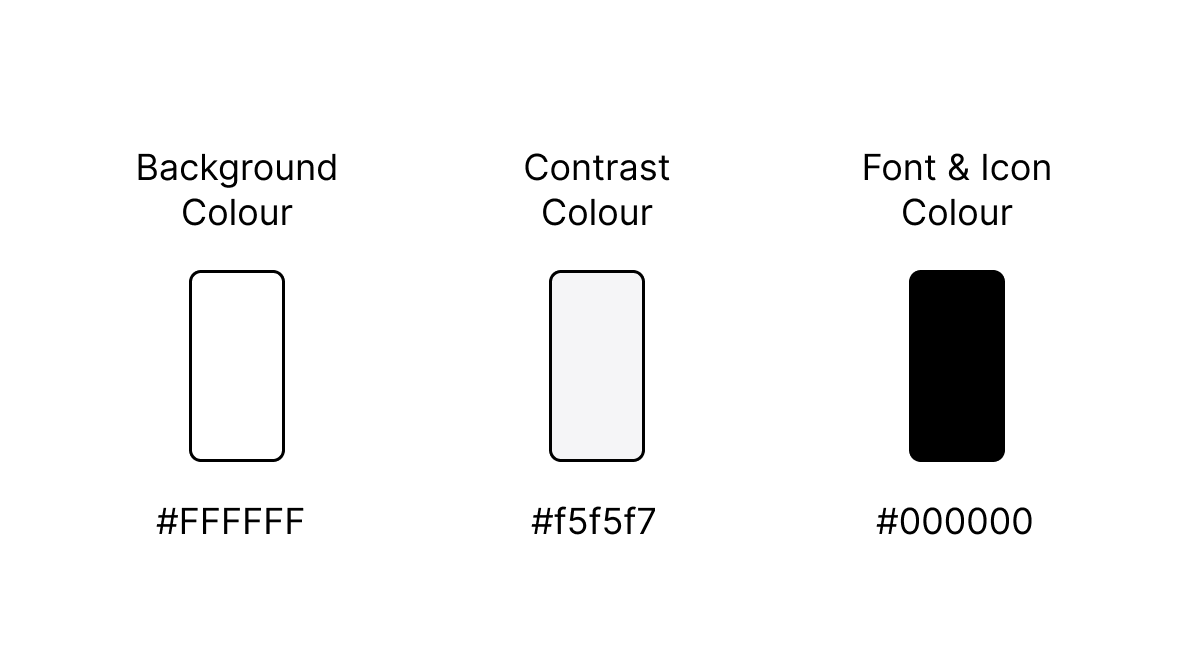
\includegraphics[width=0.4\linewidth]{figures/colors.png}
  \caption{Colour palette of the user interface.}
  \label{fig:colors}
\end{figure}

While the overall design adheres to a subdued colour palette, the visual elements within the application utilize a distinct colour scheme, as illustrated in Figure~\ref{fig:colors-dbms}. This strategic approach guarantees that charts, plots, and other visual elements command attention, supporting users to focus on those data visualisations.

\begin{figure}[h]
  \centering
  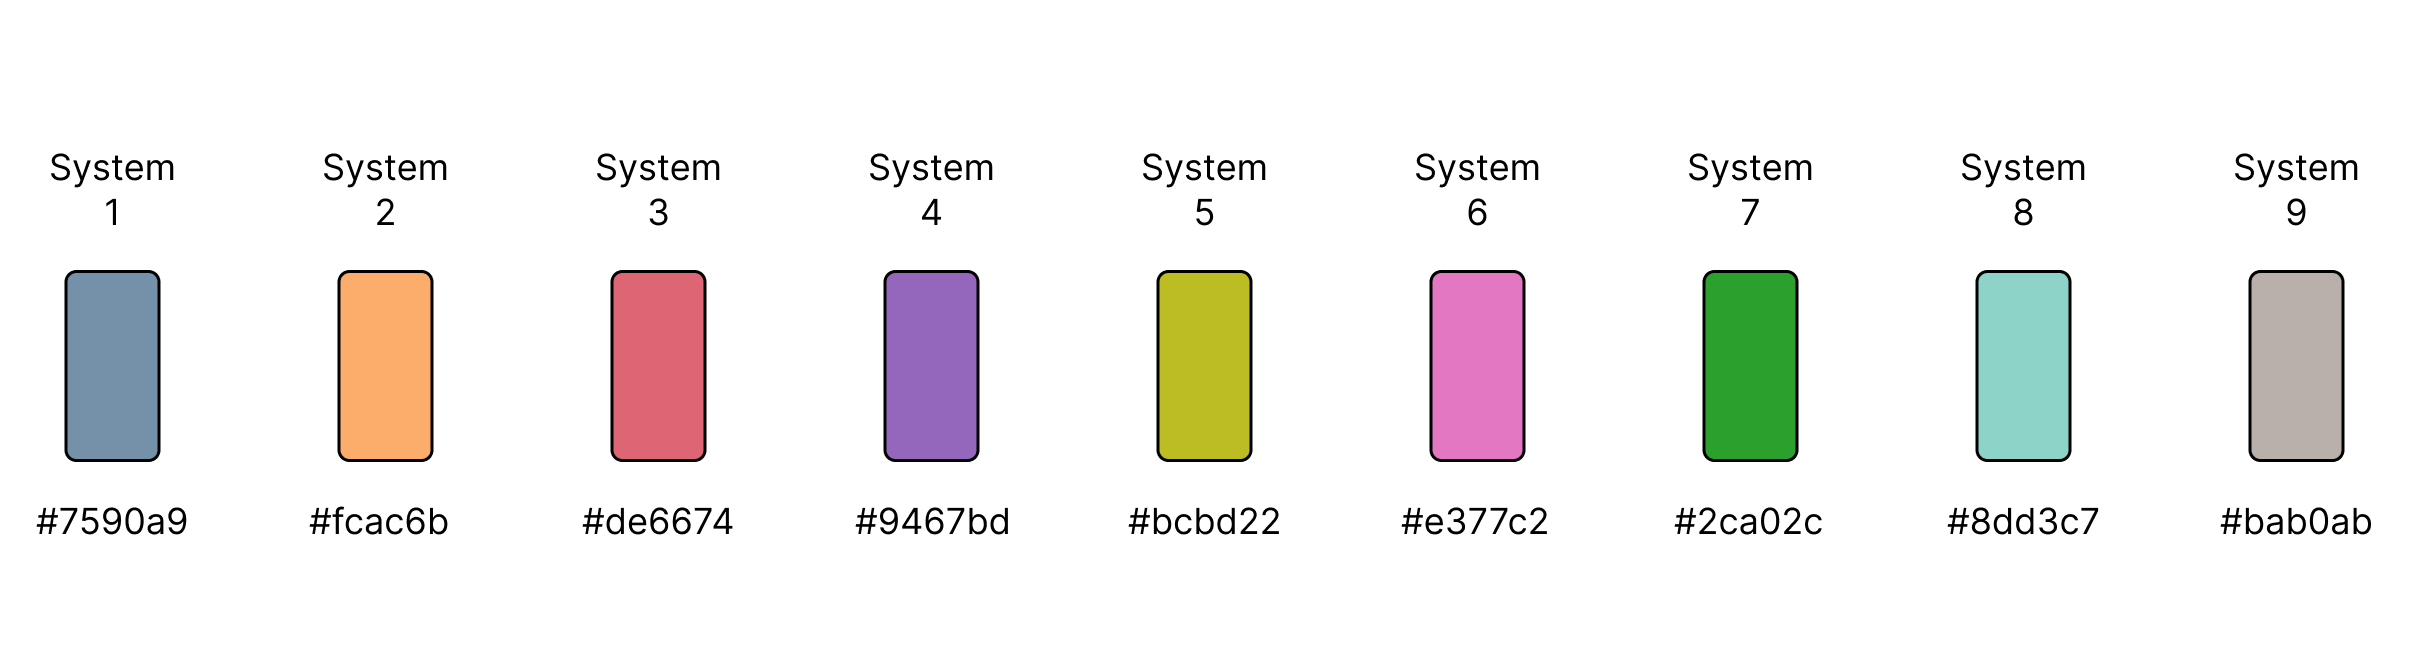
\includegraphics[width=1\linewidth]{figures/colors-dbms.png}
  \caption{Colour palette used by visualisations.}
  \label{fig:colors-dbms}
\end{figure}

To enhance user experience, the Benchy Viewer incorporates immediate feedback mechanisms. When users hover over interactive elements, such as buttons or inputs, accent colours dynamically adjust, providing a visual cue of the interactive nature of the element. Additionally, the mouse representation undergoes subtle changes, reinforcing the responsiveness of the interface.\\
Additionally, the Benchy Viewer employs the Roboto font \textcolor{red}{Zitat} for a clean and modern look, enhancing readability and contributing to a user-friendly interface.


\subsection{Page Structure and Navigation}\label{sec:page-structure}

The design of the Benchy Viewer is thoughtfully crafted for user convenience and simplicity. This section provides insights into the structural components that define the organization of the Benchy Viewer.

At the heart of the application's architecture are the header and the sidebar, ensuring constant visibility for users and facilitating seamless navigation. These elements contribute to maintaining a strong sense of orientation throughout the user journey.


\subsubsection{Sidebar}

The Benchy Viewer adopts a standard web view with a sidebar, leveraging the familiar layout seen in many web applications, as illustrated in Figure~\ref{fig:app}. This approach comes with inherent advantages. Users accustomed to web interfaces will find this structure intuitive and easily navigable, contributing to a seamless user experience.

\begin{figure}[h]
  \centering
  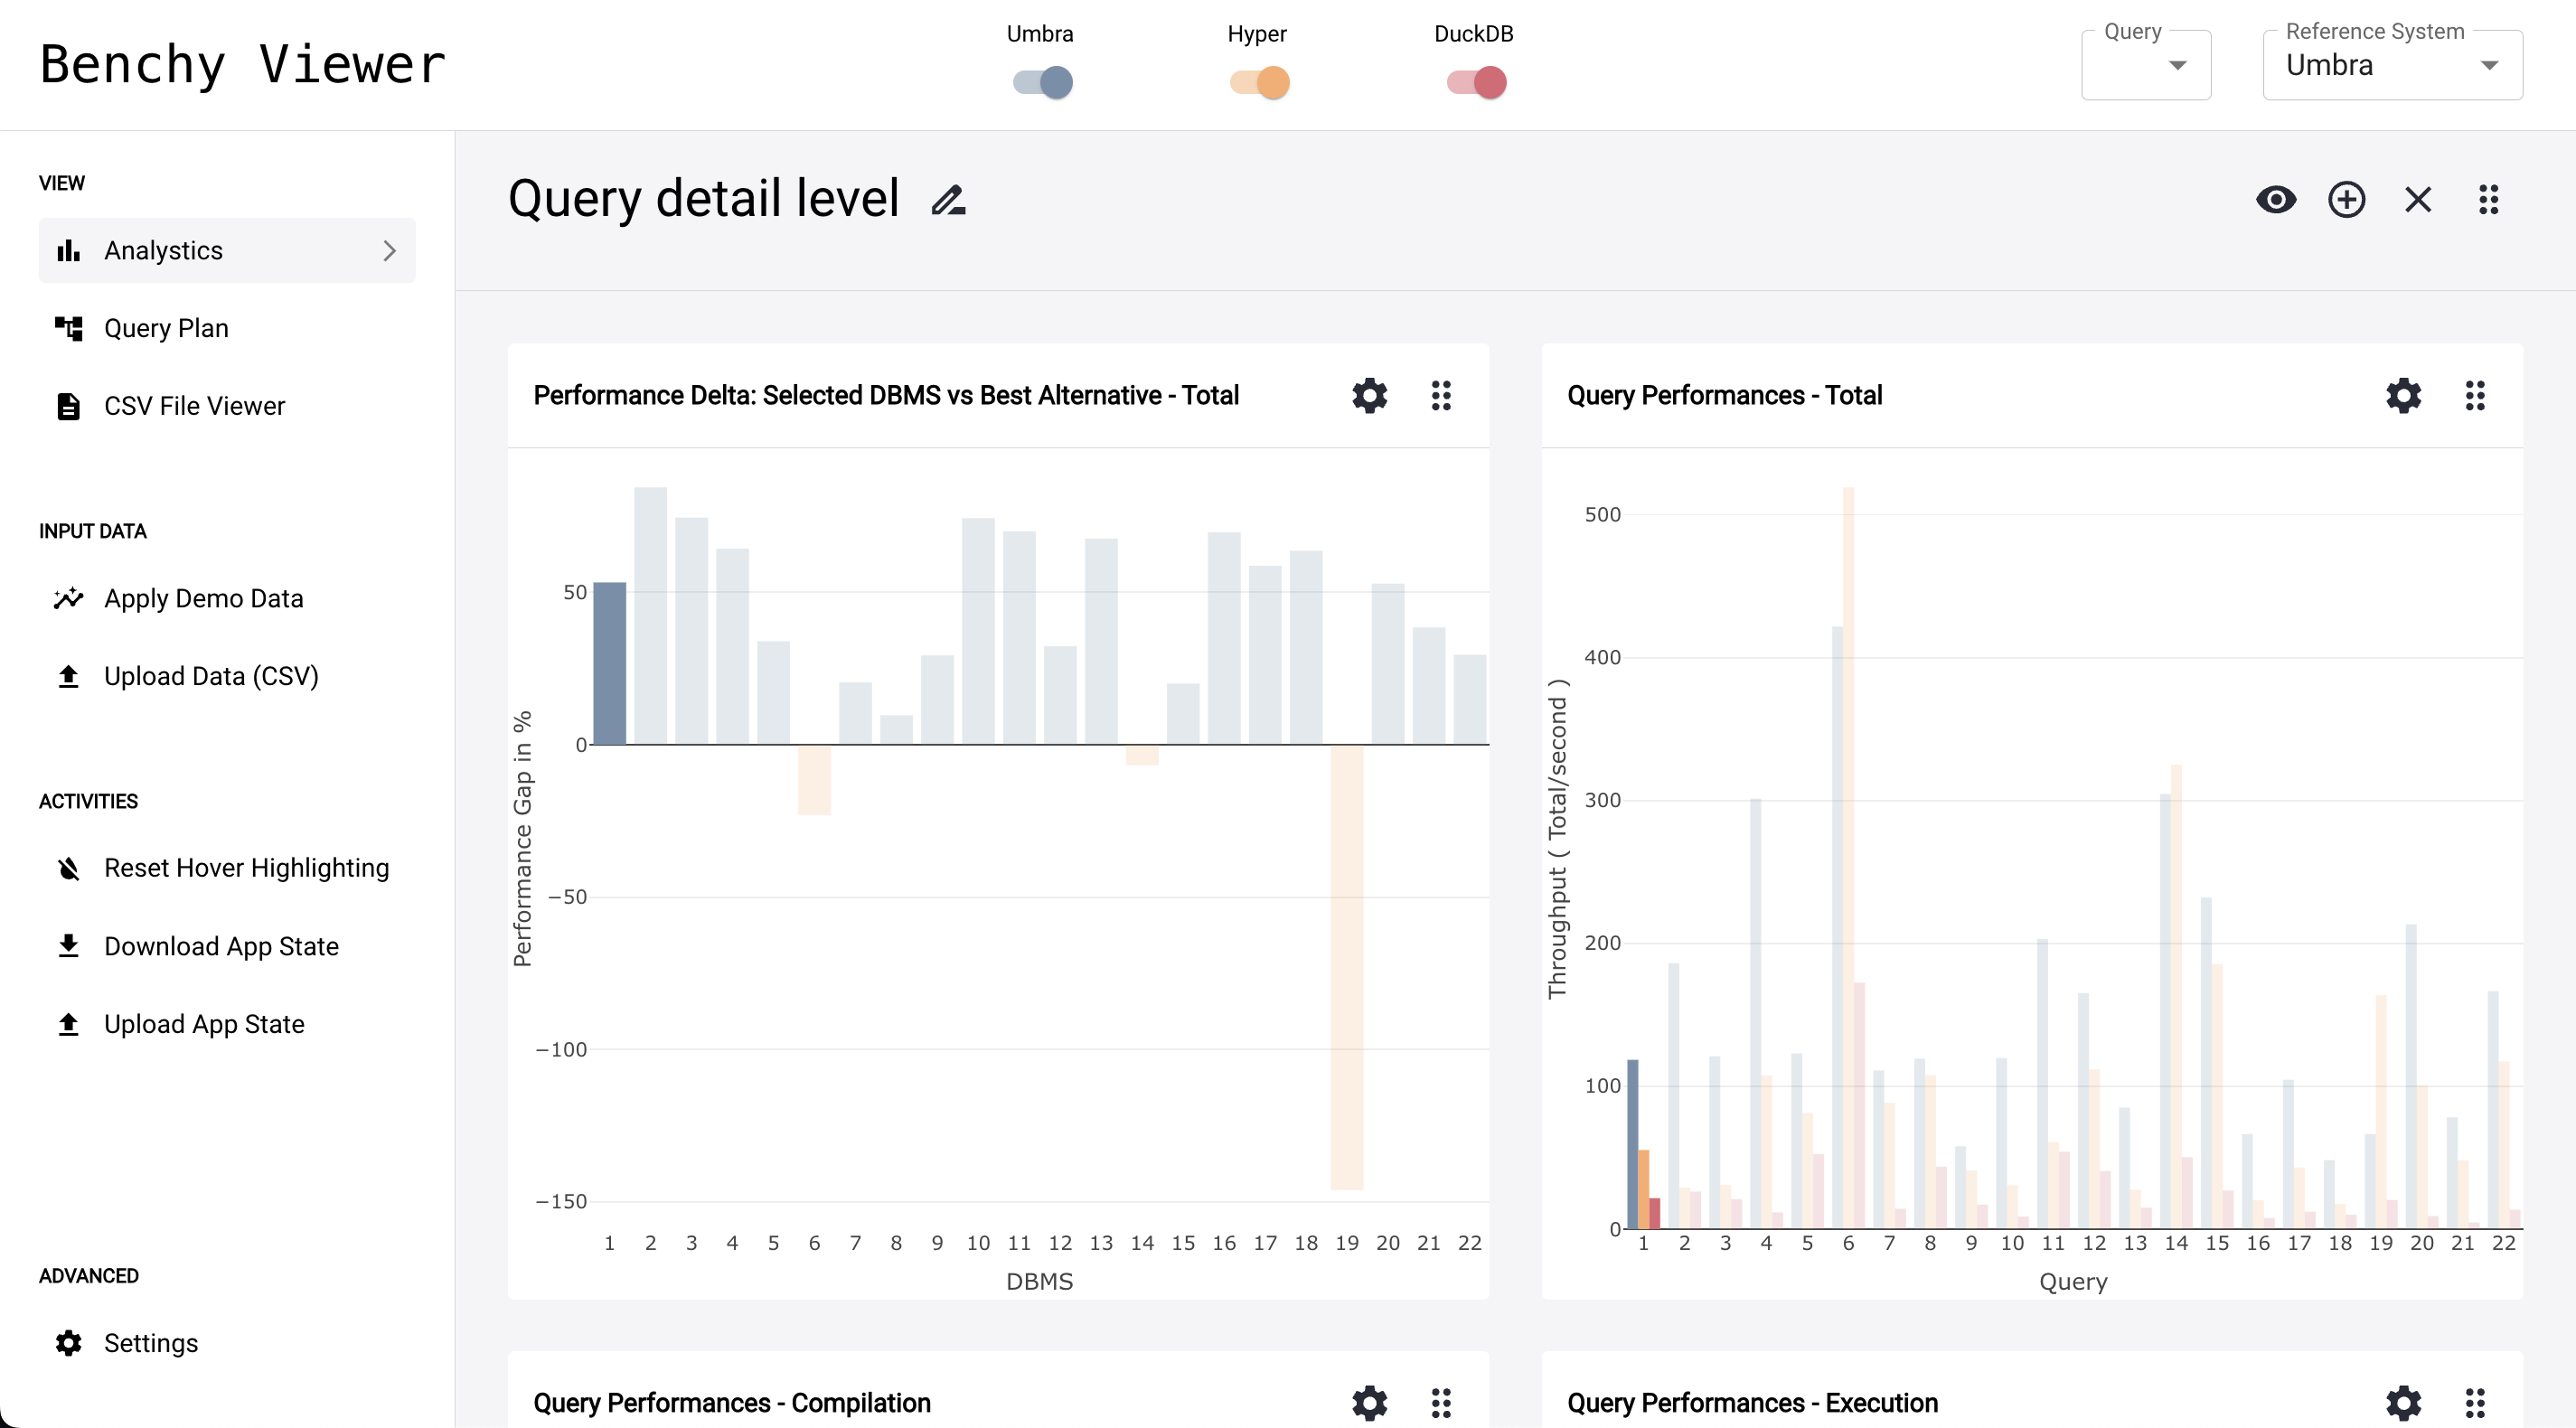
\includegraphics[width=1\linewidth]{figures/app.png}
  \caption{Overview of the application structure.}
  \label{fig:app}
\end{figure}

The sidebar serves as the central hub for navigating different sections of the application, while always staying present. By providing dedicated buttons, users can effortlessly transition between pages, ensuring quick access to specific functionalities and data views. Additionally, the navigation button of the current page is highlighted with the accent colour.

Below, the users have the possibility to import benchmark data or explore the application's capabilities using demo data. This feature facilitates a hands-on experience without the immediate need to provide personal datasets, making it convenient for users to evaluate the application's functionalities.

The sidebar offers additional functionalities, including the ability to reset hover highlighting. Users can download and upload the application state, enabling them to save configurations and share them or reload them for future sessions, which is further examined in \ref{sec:saving-sharing-state}. 

A settings icon button in the sidebar provides direct access to the global settings of the Benchy Viewer, allowing users to adjust application-wide settings from anywhere within the application.



\subsubsection{Header}
The header, along with the sidebar, remains visible in all scenarios within the Benchy Viewer. While the sidebar offers a range of functionalities, the header contains fewer elements. The central element of the header is the legend, strategically placed to eliminate the need for a legend in each individual visualisation, promoting a clean and efficient overview. Users can activate or deactivate any system at any time using the toggles within the legend.

Another crucial functionality in the header is the selection of the baseline system and the focused query, offering the same advantage of accessibility at any point in the user's workflow.

Additionally, the header adapts contextually when navigating to the "Query Plan" page. In this scenario, a slider appears for selecting the comparison strategy between query plans, providing further flexibility and control, as explored in Section \ref{sec:semantic-diff-integration}.



\subsubsection{Pages}

The Sidebar and Header form the foundation of the user interface, while the remaining space is dedicated to displaying the various pages. Essentially, the Benchy Viewer comprises three main pages, depicted in Figure~\ref{fig:pages}: the Analytics Dashboard page, the Query Plan page, and the Input File Viewer page.

\begin{figure}[h]
  \centering
  \begin{subfigure}[b]{0.3\linewidth}
    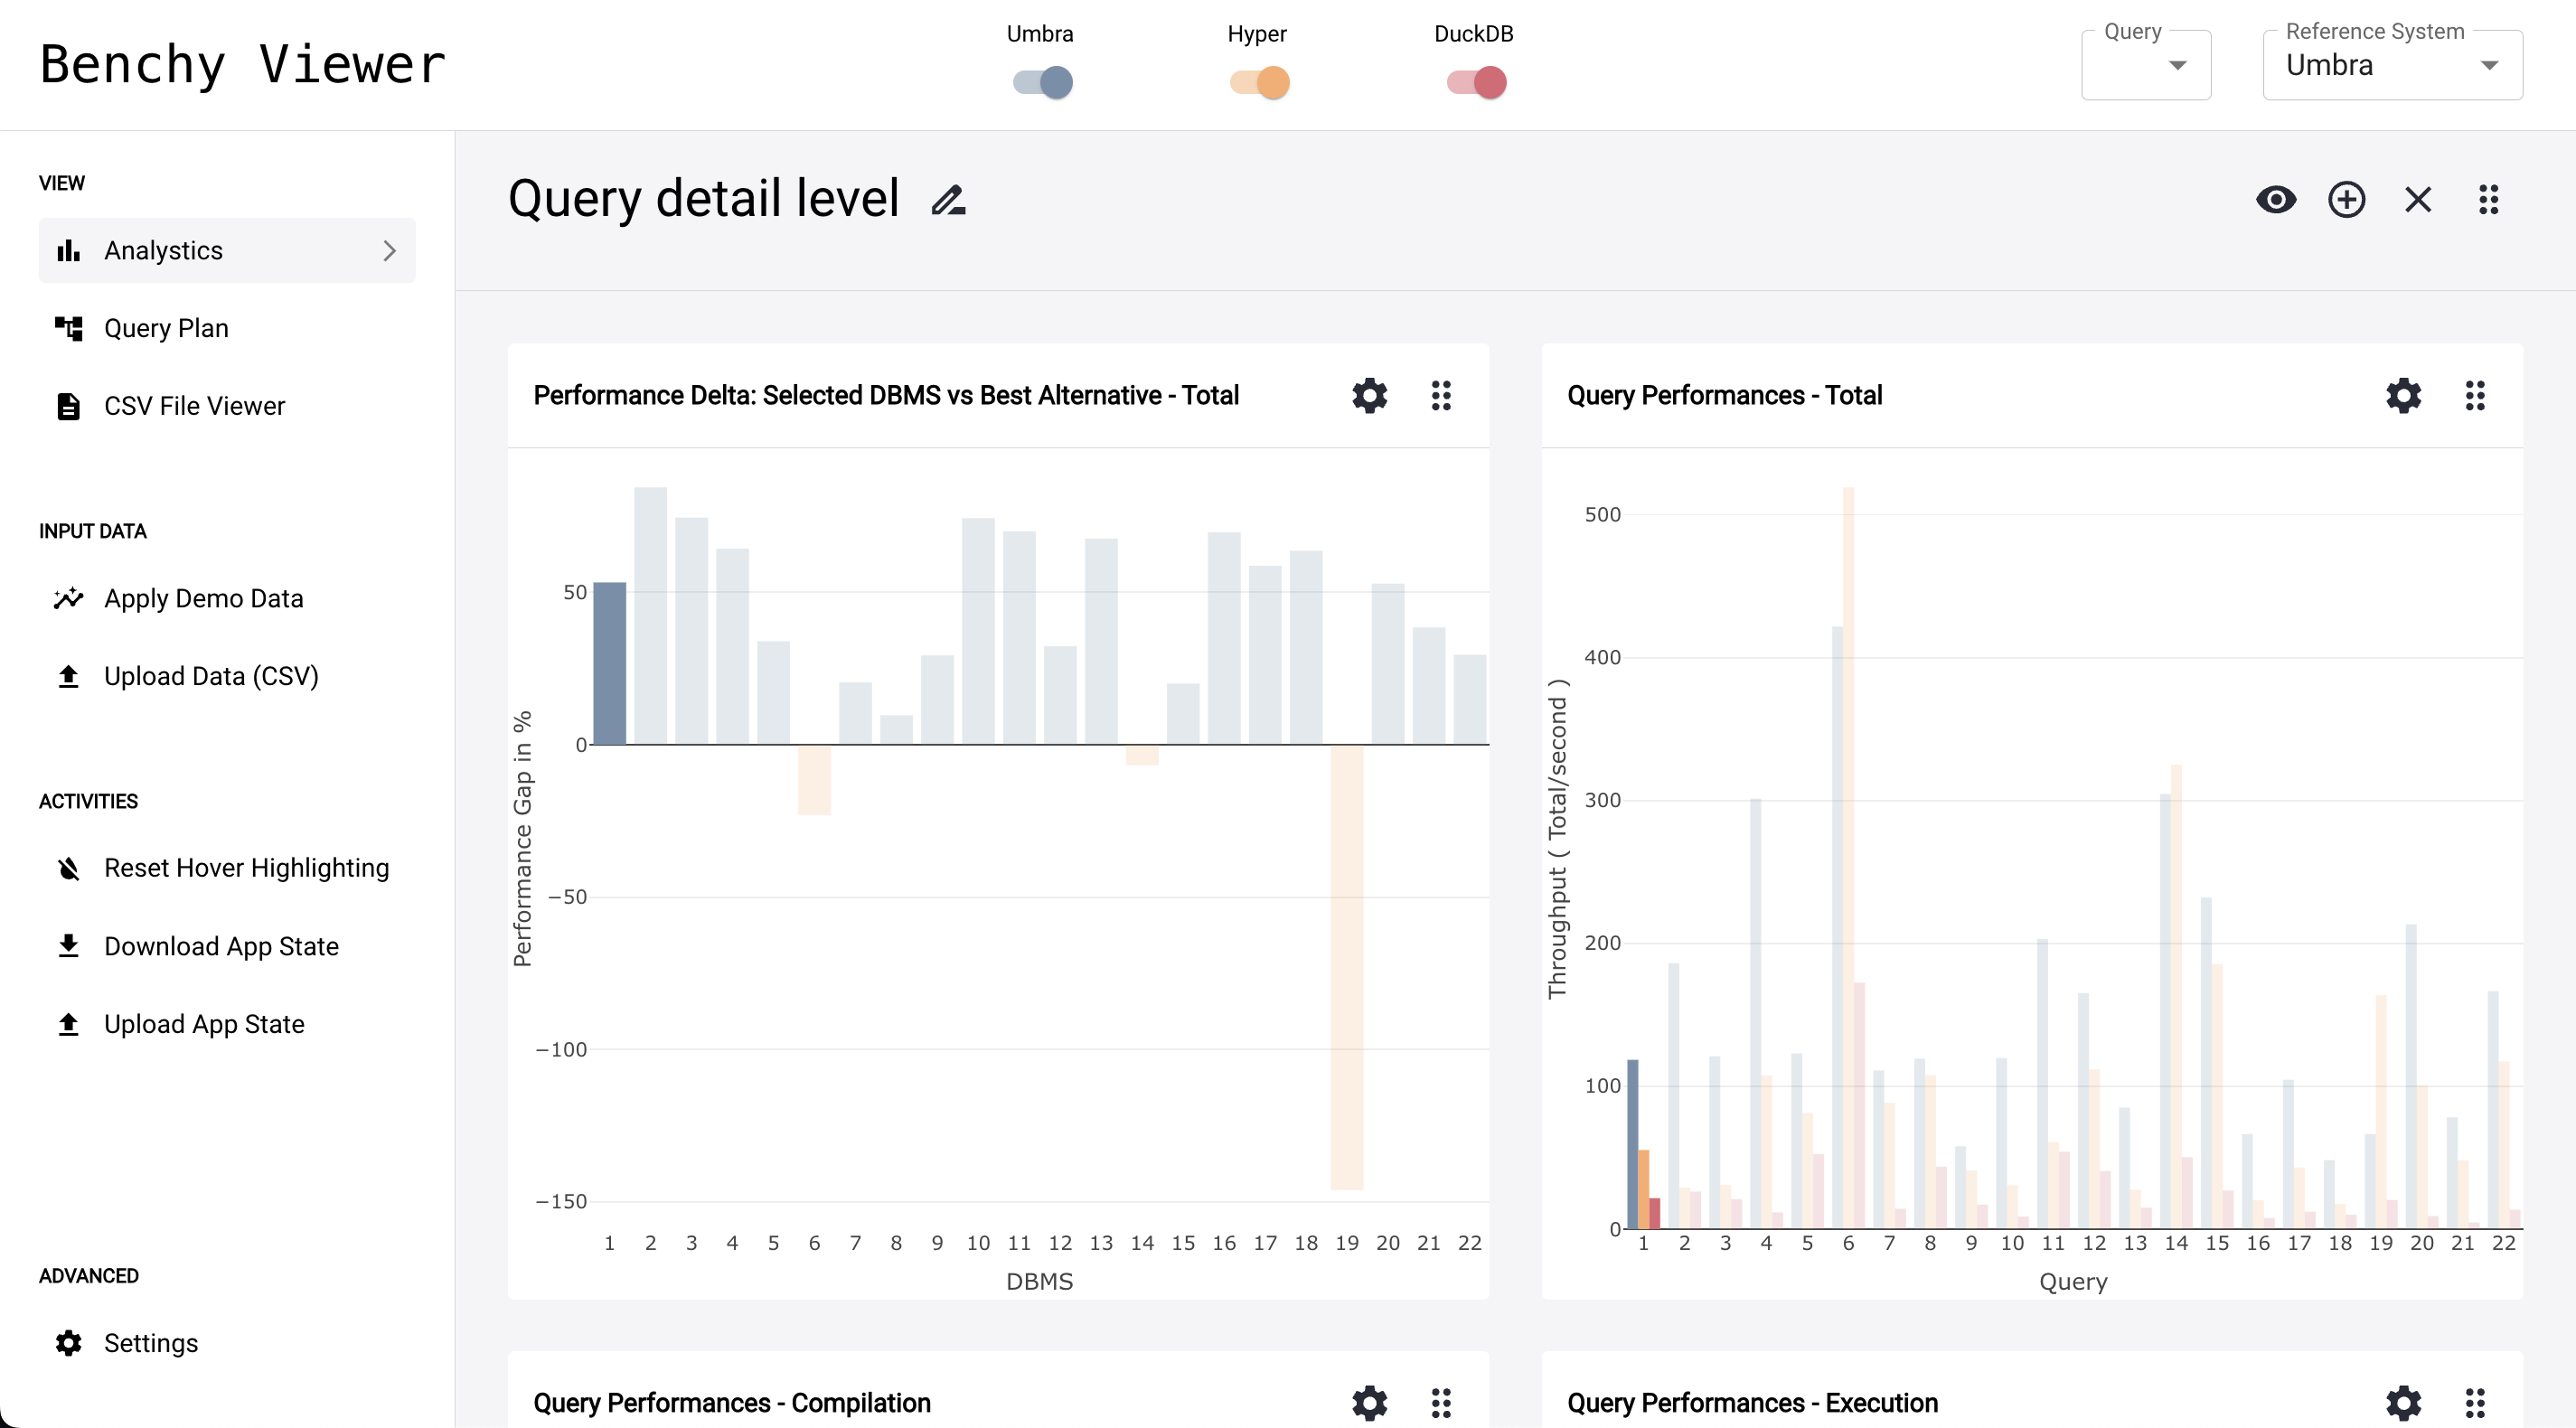
\includegraphics[width=\linewidth]{figures/app.png}
    \caption{Analytics dashboard.}
      \label{fig:app-page}
  \end{subfigure}
  \hspace{0.5cm} % Adjust the horizontal space between the figures
  \begin{subfigure}[b]{0.3\linewidth}
    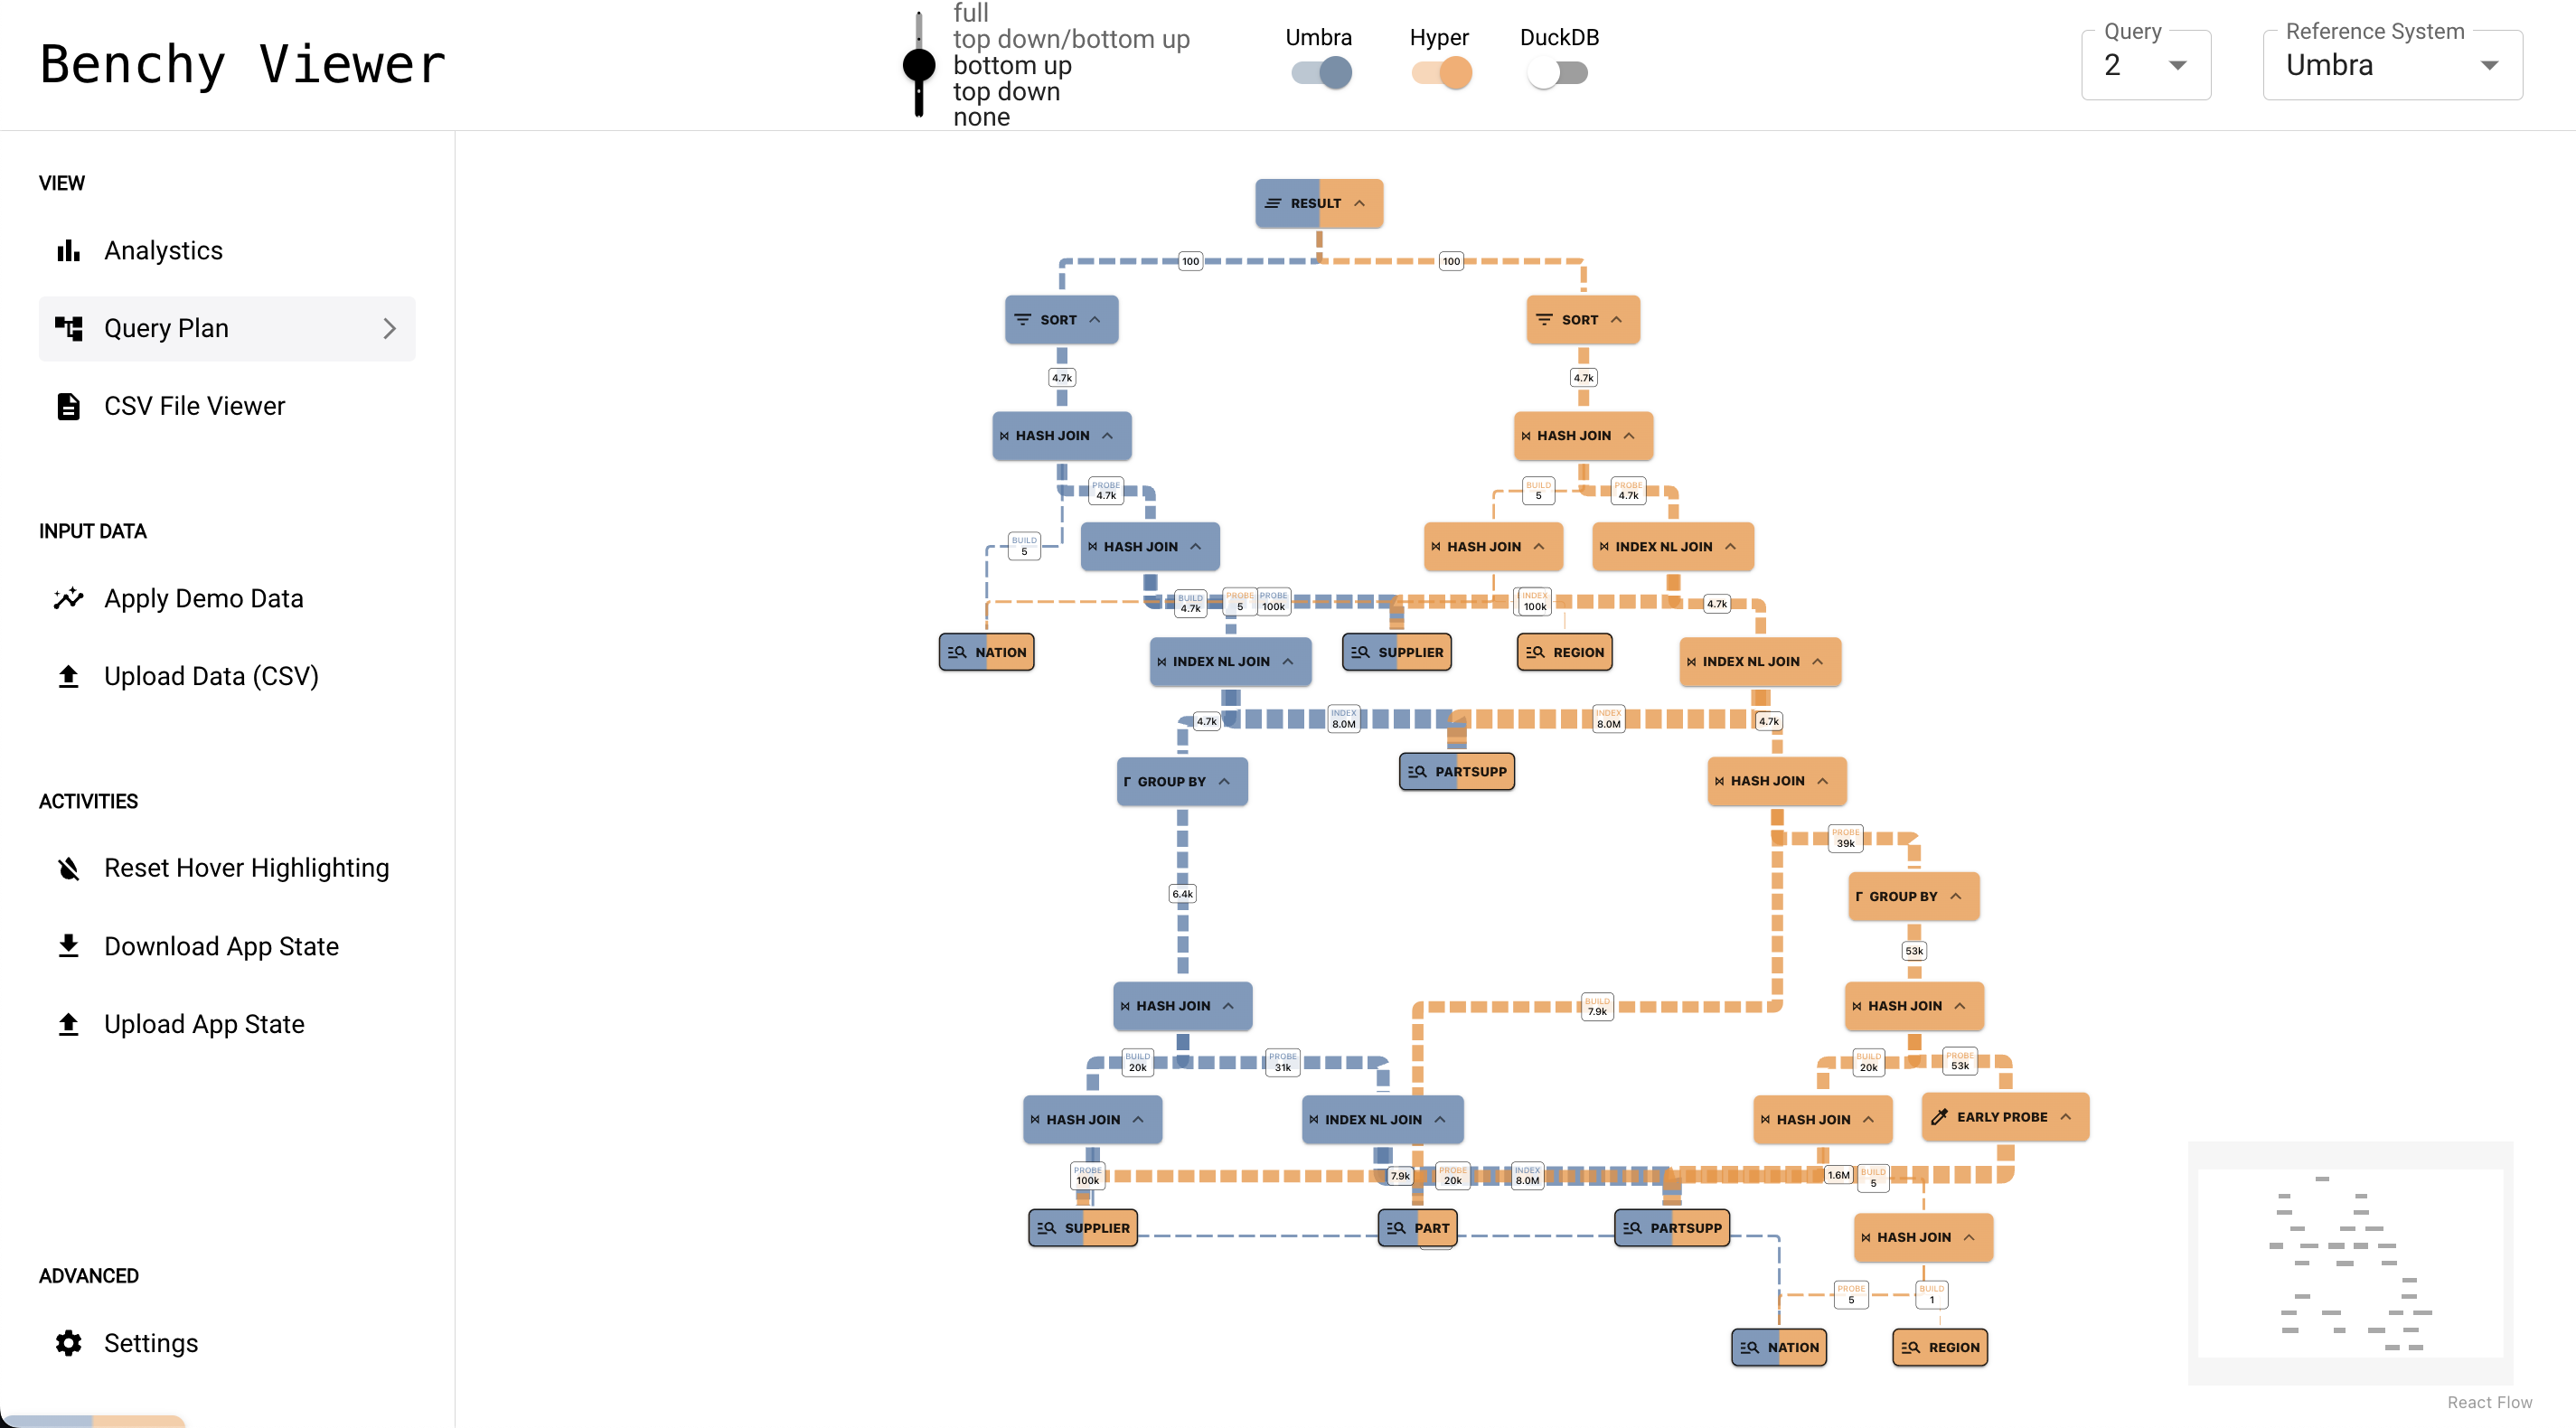
\includegraphics[width=\linewidth]{figures/app-query-plan.png}
    \caption{Query plan view.}
      \label{fig:app-query-plan}
  \end{subfigure}
  \hspace{0.5cm} % Adjust the horizontal space between the figures
  \begin{subfigure}[b]{0.3\linewidth}
    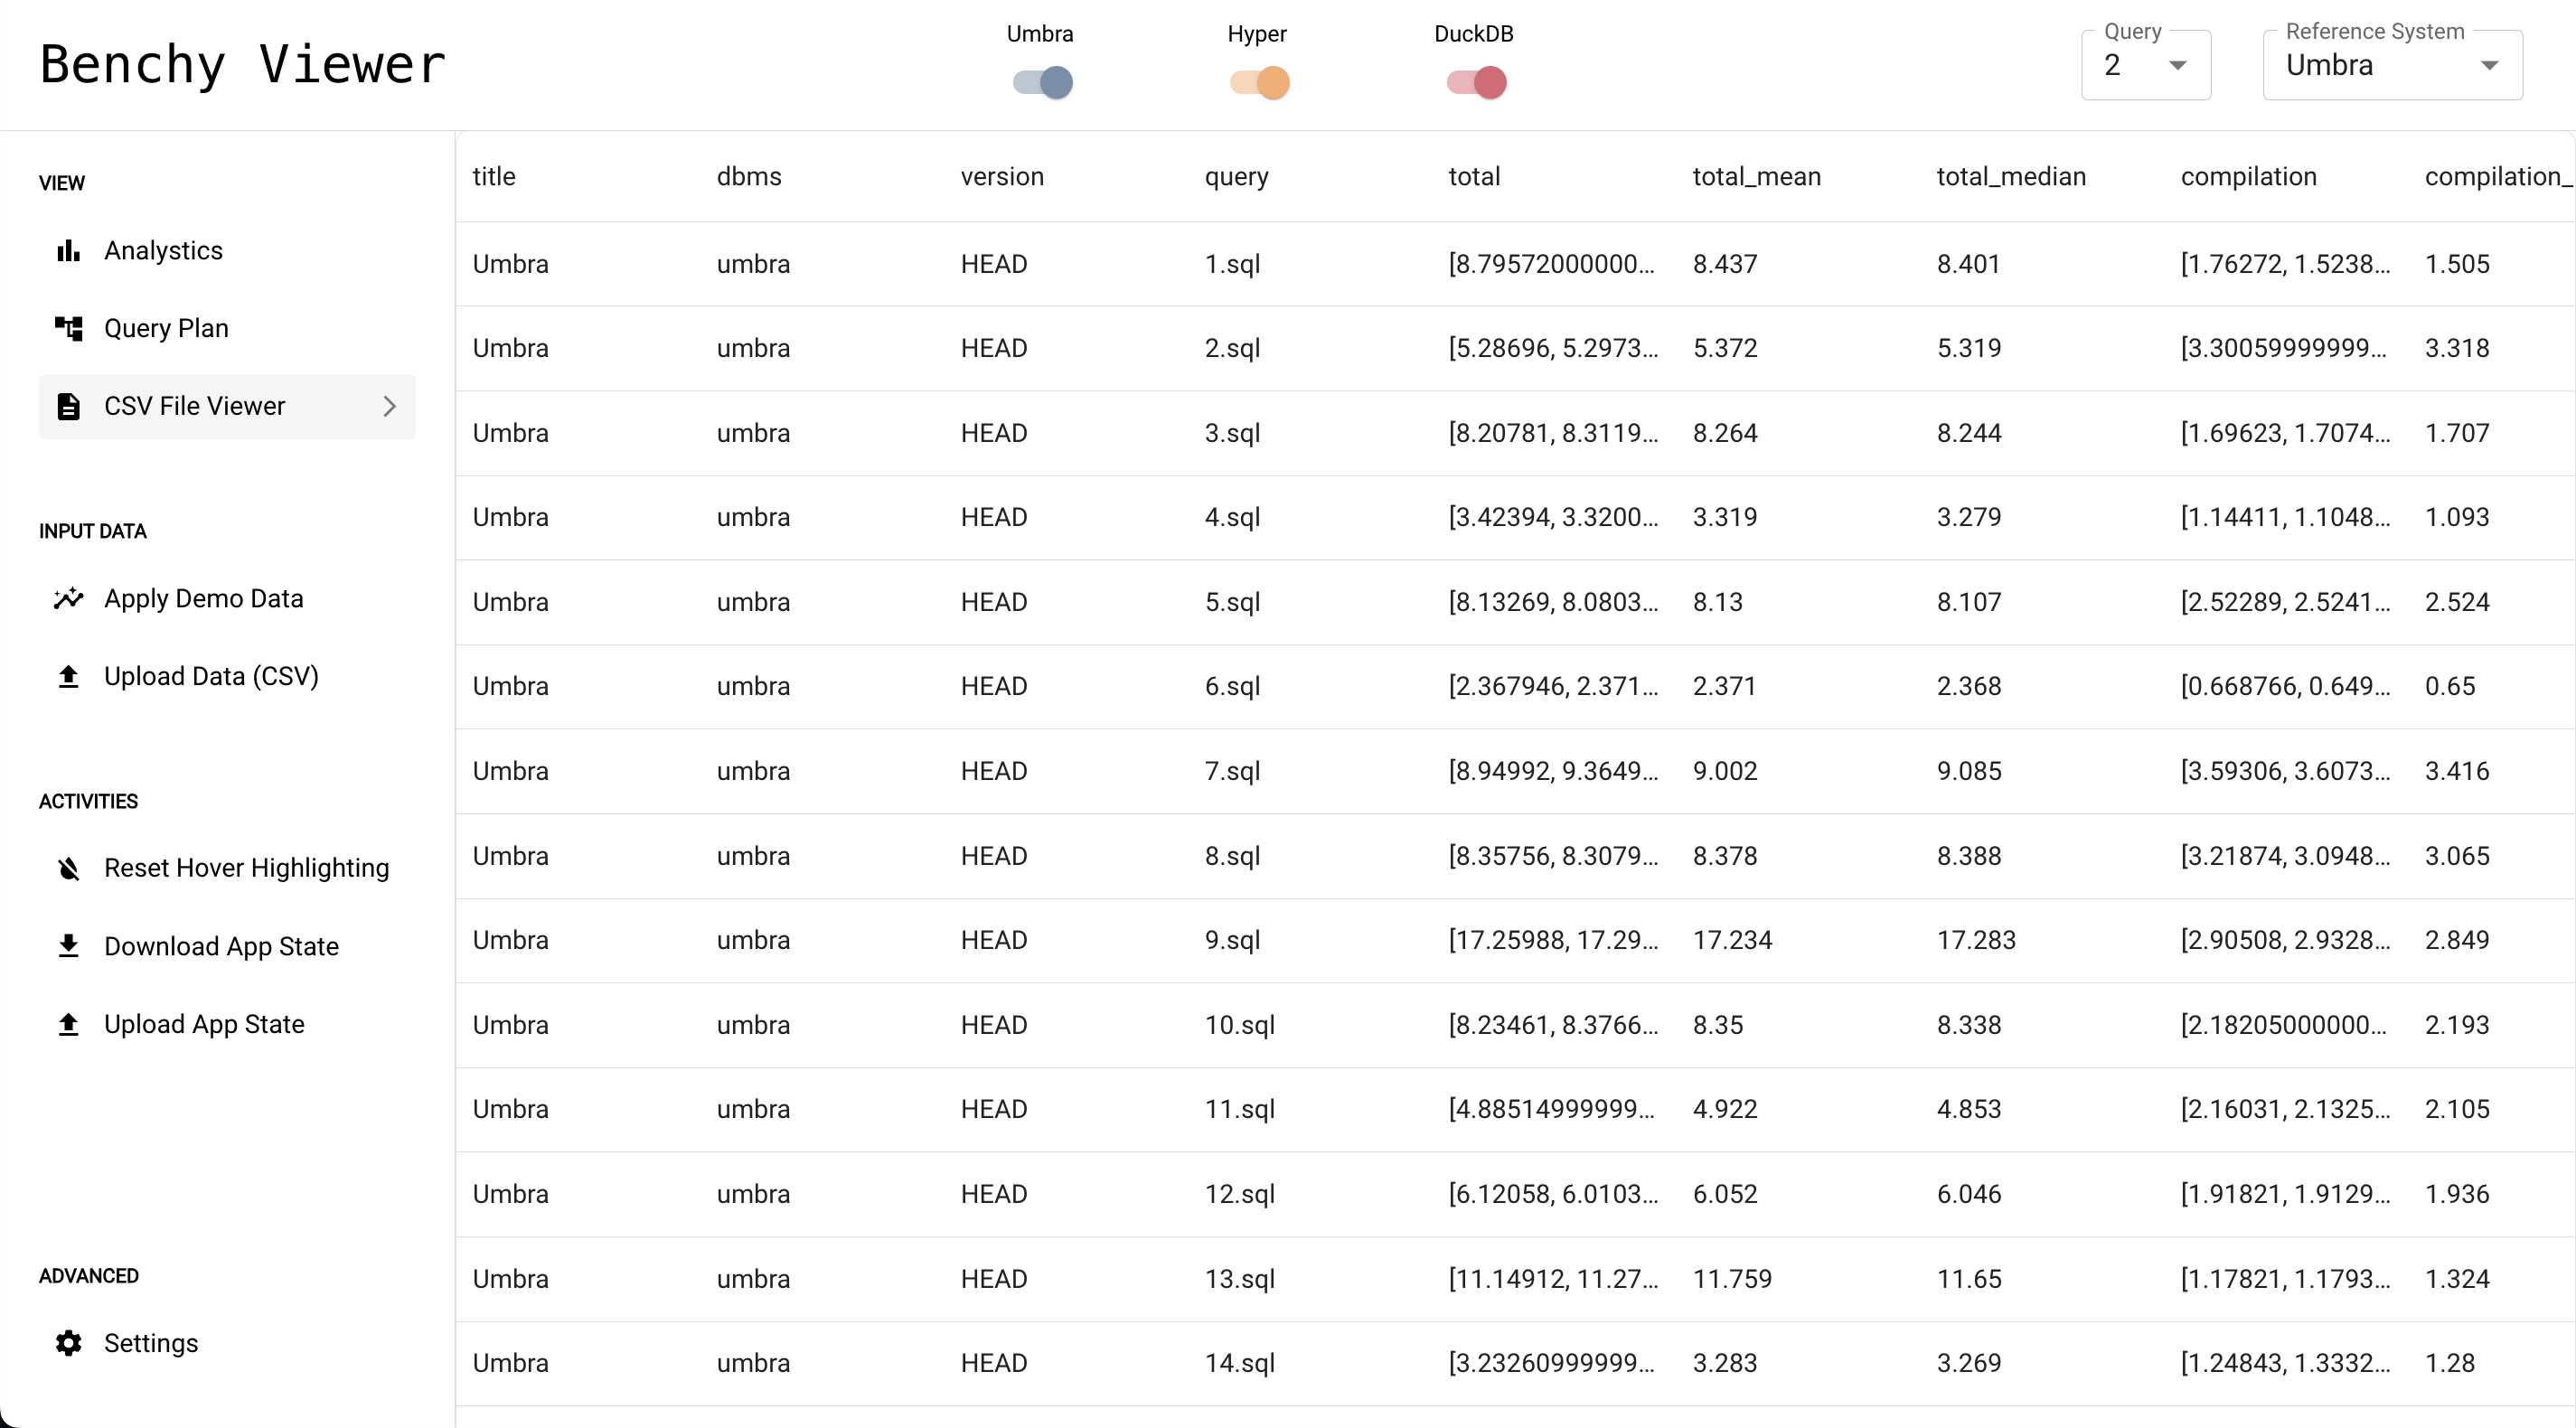
\includegraphics[width=\linewidth]{figures/app-data-viewer.png}
    \caption{Input file viewer.}
      \label{fig:app-data-viewer}
  \end{subfigure}
  \caption{From left to right: Analytics dashboard page, query plan page, and input file viewer page}
  \label{fig:pages}
\end{figure}

The Analytics Dashboard page features the drag-and-drop system for visualising elements and their containers. This page serves as the hub for analysing benchmark data, offering charts and plots to explore queries from diverse perspectives.

Upon identifying significant queries using the analytics dashboard, users often transition to the Query Plan page. This page serves as a central hub for comparing distinct query plans across various database systems. 

In contrast, the Input File Viewer page offers a minimalist perspective. Tailored for users seeking an unembellished view of their imported benchmark data, this page omits visualisations. It provides an in-depth examination of the raw data, enabling users to scrutinize the dataset's structure and intricacies without the influence of charts or plots.















\section{Data Structure}


\subsection{Overall Project Structure}

The Benchy Viewer embodies a robust project structure that leverages React, global state management, and a page navigating router, as illustrated in Figure \ref{fig:project-structure}, which we will explore in this section.

\begin{figure}[h]
  \vspace{0.5cm}
  \centering
  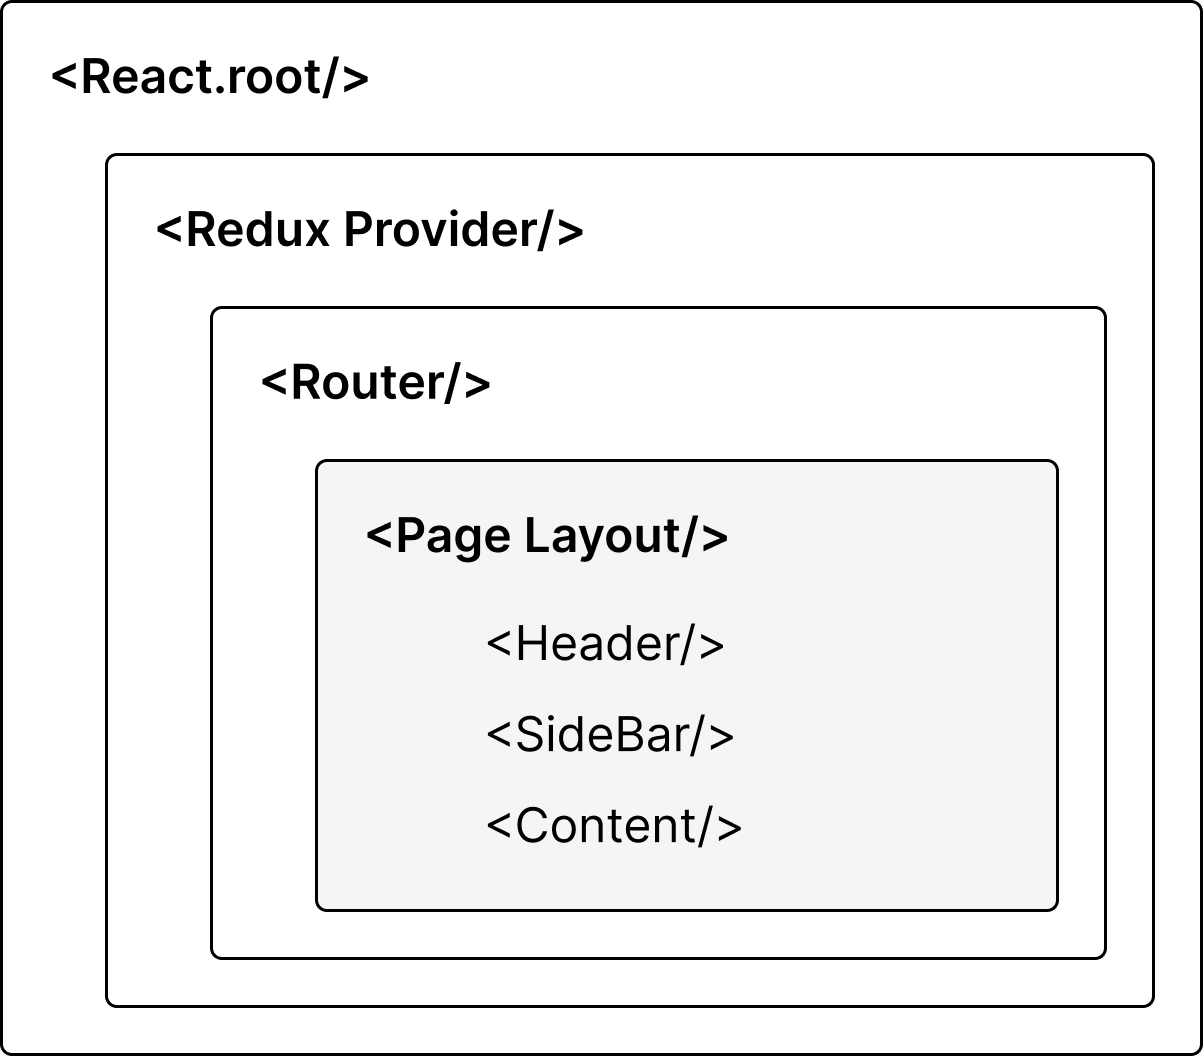
\includegraphics[width=0.5\linewidth]{figures/project-structure.png}
  \caption{Project Structure Hierarchy}
  \label{fig:project-structure}
\end{figure}

\subsubsection{Root Component}
The root component is the entry point of the Benchy Viewer React application, orchestrating critical processes that define its robustness and efficiency.\\
The primary responsibility of the root component is to render the main application, serving as the nexus for various functionalities, providing the structural and organizational backbone for the entire application. 

In the project structure hierarchy, the root component encapsulates the application with\texttt{ <React.StrictMode/>}~\parencite{reactstrictmode}, which is a tool that highlights common issues and potential problems in a React application during development.
In general, it detects impure calculations in the context of component states and multiple rendering. It enables a set of additional checks and warnings to catch and alert developers about unsafe or deprecated practices, contributing to better code quality. While it doesn't affect the production build, it's a valuable aid in identifying and addressing issues early in the development phase.


\subsubsection{State Management with Redux}
The Redux Provider in the Benchy Viewer, built using the Redux~Framework~\parencite{Redux}, serves as the central hub for managing the application's state. It acts as a shared space where different parts of the application can store and retrieve data efficiently.\\
Utilizing the capabilities of \textit{Redux Toolkit}\parencite{redux-toolkit}, the Redux Provider supplies the global state across the entire application. This global state is compartmentalized into five distinct slices, illustrated in Figure~\ref{fig:global-state}, each serving a unique purpose.

\begin{figure}[h]
  \centering
  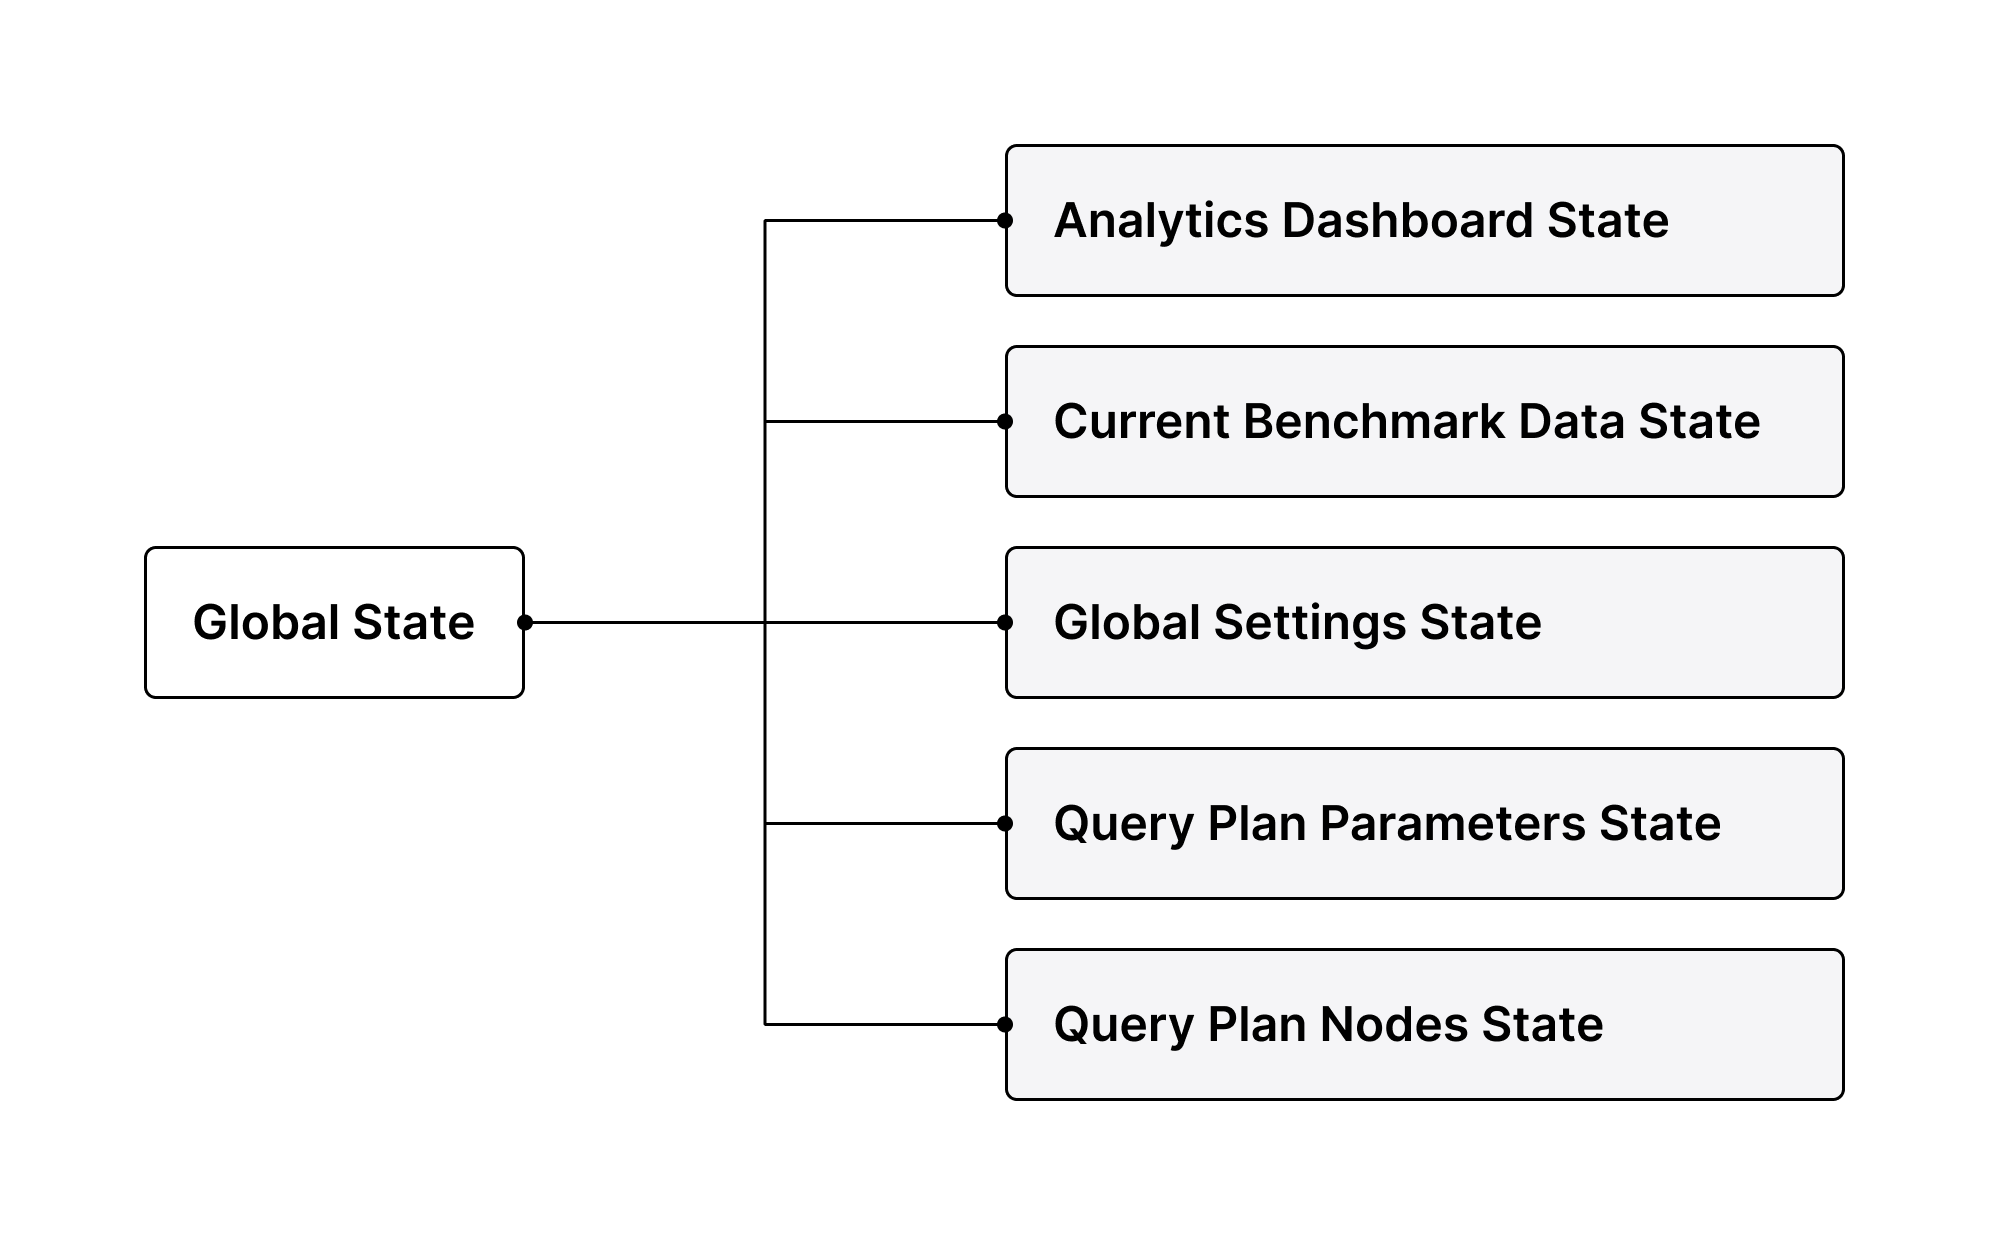
\includegraphics[width=0.8\linewidth]{figures/global-state.png}
  \caption{Application State Compartements}
  \label{fig:global-state}
\end{figure}

% Analytics Dashboard state
The Analytics Dashboard State encapsulates all the data concerning visualizations within the Analytics Dashboard. It includes information about the position within the dashboard and the configuration of each visualization element. A more detailed exploration of this data structure is provided in Section \ref{sec:analytics-dashboard}.

% Imported Benchmark Data state
The Current Benchmark Data State is responsible for holding all benchmark data from various database systems. This state is a pivotal component used across the Analytics Dashboard, Query Plan View, and Benchmark Data View. A detailed examination of this state's structure is available in Section \ref{sec:input-data}.

% Global Settings state
Focused on interactive features within visualizations, the Global Settings State encompasses functionalities like the global hover state or the selected query. Section \ref{sec:global-settings} delves into the specifics of this data structure.

% Query Plan Parameters state
Tailoring the visualization needs for the user, the Query Plan Parameters State contains data related to the appearance and comparison types of the query plans. More insights into this state are provided in Section \ref{sec:query-plan-parameters}.

% Query Plan Nodes state
Lastly, the Query Plan Nodes State unfolds the story of the actual query plan, housing details about every node and their associated information. For a comprehensive exploration, turn to Section \ref{sec:query-plan-structure}.


\subsubsection{Router}
Navigating through the corridors of the Benchy Viewer's project structure, the router, powered by \textit{React Router} \parencite{react-router}, providing a standardized approach to handle navigation in React. Specifically, in our application, this router guides users through three key areas: the Analytics Dashboard, Query Plan View, and Data Viewer.

\subsubsection{Layout and Content}
Finally, we encounter the pages with their contents within the Benchy Viewer. These pages share a consistent structure, ensuring a unified user experience. Each page adheres to a standardized layout, featuring a sidebar, a header, and a dedicated space for content, which we discussed the page structure in \ref{sec:page-structure}.

At this point, the various components at different levels come together to form the Benchy Viewer application. The root component lays the groundwork, overseeing essential processes. The Redux Provider acts as a central hub for sharing information across the application. The global state, divided into five slices, provides state to all pages. The router facilitates easy navigation between pages, which is controlled in the sidebar. In essence, these pages, with their structured layouts, unite to offer users a seamless and comprehensive experience.

\subsection{Input File and Benchmark Data}\label{sec:input-data}
% Import of Input File
% CSV Slice

% \subsubsection{Import of Performance Data}

% The first step, working with the Benchy Viewer is to import a file containing the performance data which should be visualised. The file needs to follow the format introduced in Section \ref{sec:input-file-structure}. Figure~\ref{fig:input-process-flow} summarizes the import of the input file in a process diagram.

% \begin{figure}[h]
%   \centering
%   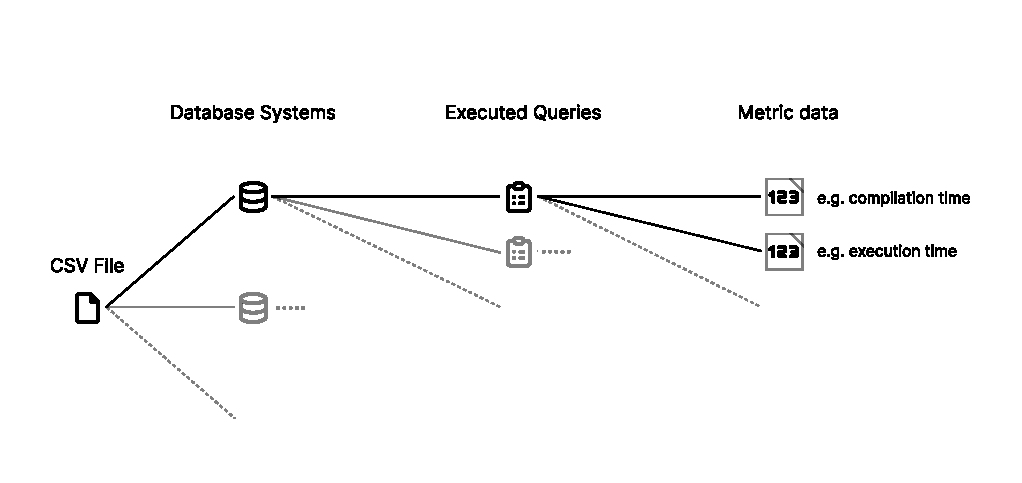
\includegraphics[width=0.2\linewidth]{figures/csv-structure.pdf}
%   \caption{Import process of input data}
%   \label{fig:input-process-flow}
% \end{figure}

% Chart beschreiben.


\subsection{Global Settings}\label{sec:global-settings}
\subsection{Analytics Dashboard Data Structure}\label{sec:analytics-dashboard}
\subsection{Query Plan}
\subsubsection{Visualisation Parameters}\label{sec:query-plan-parameters}
\subsubsection{Query Plan Data Structure}\label{sec:query-plan-structure}















\section{Integration of Plotly-React for Data Visualisation}
\subsection{Types of Plots and Charts}
\subsection{Hover Feature}
\subsection{Selected Query Feature}

\section{Integration of semantic-diff-tool}\label{sec:semantic-diff-integration}
\subsection{Business Logic}
\subsection{Settings}
\subsection{UI}